\subsection{Vision Transformer}\label{s:vit}
\chapterauthor{Low Hong Sheng Jovian (2203654)}

Vision Transformers (ViT) mark a crucial adaptation of transformer architectures from textual to image analysis \cite{Khan2021Transformers}. Initially designed for natural language processing, transformers employ self-attention mechanisms which are adeptly applied to visual data in ViTs. This adaptation enables the model to dynamically prioritize different image segments according to their relevance for tasks like tumor detection in brain MRI scans.

ViTs work by breaking down an image into fixed-size patches, embedding them linearly, and treating each as a token, similar to words in text processing \cite{Wu2020Visual} (see Figure \ref{fig:vit_architecture}). Positional embeddings are added to maintain spatial relationships. These embeddings are processed through multiple transformer layers, utilizing self-attention to analyze the image holistically, enhancing the detection of complex patterns and subtle nuances indicative of tumors.

\begin{figure}[H]
  \centering
  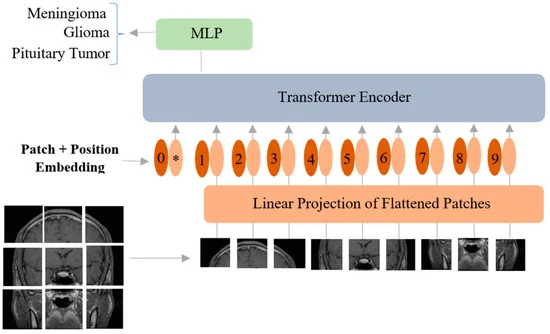
\includegraphics[width=0.45\textwidth]{vit/vit_architecture.png}
  \caption{ViT Architecture \cite{curroncol29100590}}
  \label{fig:vit_architecture}
\end{figure}

This method allows ViTs to excel in scenarios requiring deep contextual understanding and detailed image analysis. Particularly in medical imaging, ViTs are highly effective, often surpassing conventional CNNs by identifying less obvious features crucial for accurate diagnostics \cite{Matsoukas2021Is}.

Additionally, ViTs benefit from transfer learning, where models pre-trained on extensive general datasets are fine-tuned for specific medical tasks \cite{Simon2022Vision}. This not only reduces the need for large medical datasets but also speeds up the training process. Their adaptability and prowess in handling intricate image data make Vision Transformers a promising advancement in medical diagnostics, especially for improving the accuracy and reliability of brain tumor classifications.


\subsubsection{Vision Transformer Data Preprocessing}

In the initial stages of this project, several preprocessing steps were considered to optimize the performance of the ViT model for brain MRI classification. Typically, the ViT model benefits from breaking down images into smaller patches, as this allows the self-attention mechanism to effectively capture local and global features within the image. For this reason, the dataset was initially preprocessed to create patches from 224x224 pixel images. This preprocessing included resizing, cropping, normalization, and dividing the images into smaller patches.

However, during experimentation, it was observed that this approach did not yield the desired performance improvements. Specifically, the model's accuracy and ability to generalize did not improve significantly when using patched images. This was likely due to the relatively small size of the dataset, which limited the model's capacity to effectively learn from the patches. 

\begin{figure}[H]
  \centering
  \begin{subfigure}[b]{0.30\textwidth}
      \centering
      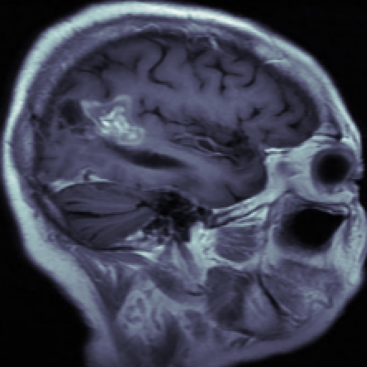
\includegraphics[width=\textwidth, height=3.5cm]{vit/vit_patch_og.png}
      \caption{Original Glioma Image before Patching}
      \label{fig:vit_patch_og}
  \end{subfigure}
  \hfill
  \begin{subfigure}[b]{0.30\textwidth}
      \centering
      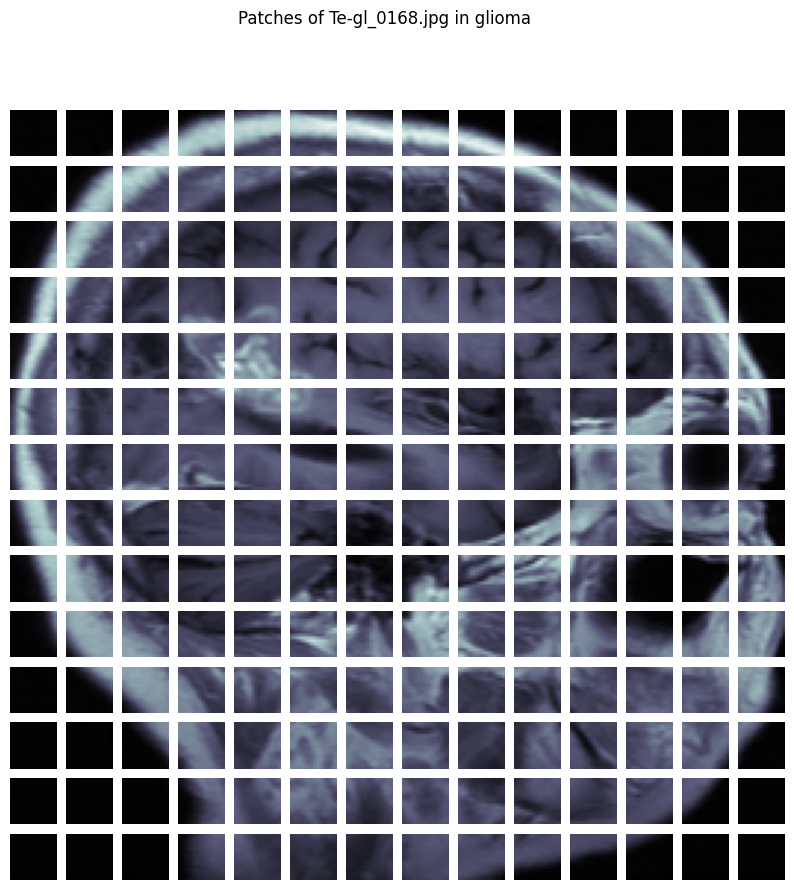
\includegraphics[width=\textwidth, height=3.5cm]{vit/vit_patch.png}
      \caption{$16x16$ Sample Patches of the Glioma Image}
      \label{fig:vit_patch}
  \end{subfigure}
  \hfill
  \begin{subfigure}[b]{0.30\textwidth}
      \centering
      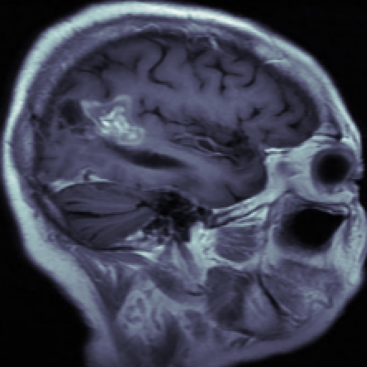
\includegraphics[width=\textwidth, height=3.5cm]{vit/vit_patch_img.png}
      \caption{$16x16$ Sample of the Reconstructed Glioma Image}
      \label{fig:vit_patch2}
  \end{subfigure}
  \caption{Comparison of $16x16$ Image Patching: (a) Original Image, (b) Sample Patches, (c) Patched Image}
  \label{fig:vit_patches}
\end{figure}

Figure \ref{fig:vit_patches} illustrates the image patching process. The first image (a) shows the original glioma image before any modifications. The second image (b) illustrates the same image divided into $16x16$ patches, revealing how it is segmented into smaller parts. The third image (c) presents a sample of the reconstructed glioma image from these patches, showcasing the reassembly process. This patching technique is crucial for Vision Transformers, as it enables the model to examine different segments of the image using the self-attention mechanism.

However, employing the typical 16x16 patch size for ViT models \cite{Wang2021Not} significantly increased computational complexity. Each 224x224 pixel image was divided into 196 patches (see Fig \ref{fig:vit_patch}), and with a dataset of 480 images, the resulting number of patches became too large to handle, even when upgraded to Google Colab Pro. This vast number of patches overwhelmed the system's memory and processing capabilities, severely impeding the training process.

As a result, the preprocessing strategy was adjusted to utilize the pretrained ViT model directly on the original 224x224 pixel images. This change balanced computational efficiency and model performance, making the training process feasible given the hardware constraints and dataset size.


\subsubsection{Implementation}

The proposed brain MRI classification model employs the ViT architecture, specifically the B16 variant, pretrained on the ImageNet dataset. The Vision Transformer represents a significant departure from traditional convolutional neural network models like InceptionV3, U-Net, and ResNet-50, primarily through its utilization of self-attention mechanisms. These mechanisms enable ViT to effectively capture and interpret the global context of an image, a capability that proves particularly valuable in the domain of medical image analysis, such as MRI scans. Unlike conventional models that rely on local receptive fields, ViT assesses all parts of the image in relation to one another, enhancing the detection and classification of nuanced features within complex medical images.

To specifically tailor the ViT model for brain MRI classification, several key adjustments were made. Initially, an input size of 512x512 pixels was used; however, this did not result in good performance of the model. Consequently, the input size was adjusted to 224x224 pixels with three channels, aligning with the common dimensions of medical imaging datasets. The B16 variant of the Vision Transformer was employed without its original classification head. 

\begin{figure}[H]
  \centering
  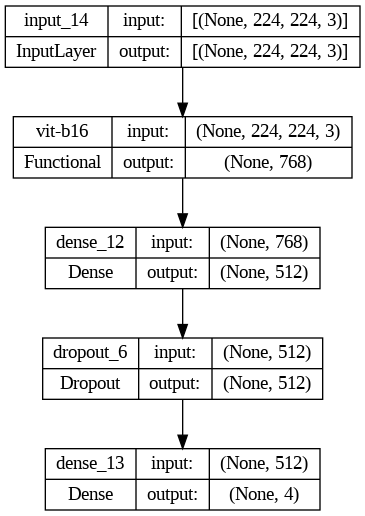
\includegraphics[width=0.30\textwidth, height=4.2cm]{vit/vit_architecture2.png}
  \caption{ViT Implemented Architecture}
  \label{fig:vit_implemented_architecture}
\end{figure}

The implemented architecture of the model is visually represented in Figure \ref{fig:vit_implemented_architecture}. It begins with an input layer that accepts images with dimensions 224x224 pixels and 3 channels (RGB). It then employs the Vision Transformer (ViT) B16 variant, which processes the input image and generates an output feature map with 768 dimensions, effectively capturing essential features while reducing dimensionality. This output is passed through a dense (fully connected) layer with 512 neurons, which helps in learning complex representations from the feature map. To mitigate overfitting, a dropout layer with a rate of approximately 32.8\% is applied next, randomly setting a fraction of input units to zero at each update during training. The final layer is another dense layer with 4 neurons, each corresponding to one of the four brain tumor classes, using a softmax activation function to convert the outputs into probabilities. This sequential architecture effectively captures and processes essential features from the input images, facilitating accurate classification of brain MRI scans into the specified tumor classes.

Typically, the output layer of ViT uses a Multi-Layer Perceptron (MLP) layer as shown in Figure \ref{fig:vit_architecture}. However, since the dataset provided is very small and ViT models are generally used for very large datasets, a softmax activation function was used instead. The softmax function is advantageous in this context because it converts the output logits into probabilities that sum to one, which is particularly useful for multi-class classification problems. This provides a clear probabilistic interpretation of the model's predictions, making it easier to identify the most likely class for each input image. The final classification layer, therefore, utilizes a softmax activation function to provide the probabilities for each class, enhancing the model's ability to make accurate predictions on diverse MRI data.

The model training and optimization involved several critical steps. The model leverages a custom Adam optimizer with a learning rate of approximately 0.0001, based on its empirical effectiveness in similar tasks involving high-dimensional image data. This choice ensures stable and gradual adjustments to the weights. The categorical cross-entropy loss function was utilized to address the multi-class nature of the classification challenge, ensuring effective discrimination between different brain tumor types. 

Training extended over 50 epochs with an early stopping mechanism that ceased training if there was no improvement in validation loss over 10 consecutive epochs. The optimal model was preserved and further assessed on a validation set, achieving a peak training accuracy of 1.000 and a validation accuracy of 0.9375 with the lowest validation loss recorded at 0.3430.


\subsubsection{Fine-Tuning}

To fine-tune the ViT model, several advanced techniques and tools were employed to optimize its performance for brain MRI classification. Initially, the batch size was systematically varied to identify the optimal setting for our specific task. After testing different batch sizes, it was determined that a batch size of 16 yielded the best performance, aligning with common practices in training Vision Transformer models \cite{Al-Hadhrami2023An}. This batch size struck a balance between computational efficiency and model accuracy, enhancing the model's ability to learn from the data without overfitting or underfitting.


In an effort to enhance the ViT model's performance for brain MRI classification, several techniques were explored. L2 regularization was applied to prevent overfitting by penalizing large weights, and some layers of the pre-trained ViT model were frozen to retain their learned features while fine-tuning the final layers. However, these approaches did not improve the model's ability to accurately classify the four classes. Consequently, they were not included in the final model's implementation.

To determine the most effective hyperparameters, the Optuna package was utilized, specifically optimizing the learning rate and dropout rate. Additionally, the training process incorporated early stopping to prevent overfitting, checkpointing to save the best model based on validation loss, and learning rate reduction on plateau to dynamically adjust the learning rate during training. These strategies collectively enhanced the model's performance and robustness, ensuring accurate classification of brain MRI scans.

Table \ref{tab:vit_finetune1} and \ref{tab:vit_finetune2} summarizes the results of the fine-tuning trials, listing the validation loss for each tested dropout rate and learning rate.

\begin{table}[H]
  \begin{minipage}{0.45\textwidth}
    \centering
    \begin{longtable}{|c|c|c|}
      \caption{Fine-Tuning Results for Different Dropout Rates}\label{tab:vit_finetune1} \\
      \hline
      \textbf{Trial} & \textbf{Dropout Rate} & \textbf{Validation Loss} \\
      \hline
      \endfirsthead
      \caption[]{Fine-Tuning Results for Different Dropout Rates (continued)}\\
      \hline
      \textbf{Trial} & \textbf{Dropout Rate} & \textbf{Validation Loss} \\
      \hline
      \endhead
      \hline
      \endfoot
      \hline
      \endlastfoot
      Trial 1 & 0.3154 & 0.6655 \\
      \hline
      Trial 2 & 0.3336 & 0.5207 \\
      \hline
      Trial 3 & 0.3160 & 0.5524 \\
      \hline
      Trial 4 & 0.3276 & 0.3425 \\
      \hline
      Trial 5 & 0.3962 & 0.4133 \\
      \hline
      Trial 6 & 0.3459 & 0.5437 \\
      \hline
      Trial 7 & 0.3640 & 0.6166 \\
      \hline
      Trial 8 & 0.3779 & 0.4895 \\
      \hline
      Trial 9 & 0.3845 & 0.6720 \\
      \hline
      Trial 10 & 0.3186 & 0.5634 \\
      \hline
    \end{longtable}
  \end{minipage}
  \hfill
  \begin{minipage}{0.45\textwidth}
    \centering
    \begin{longtable}{|c|c|c|}
      \caption{Fine-Tuning Results for Different Learning Rates}\label{tab:vit_finetune2} \\
      \hline
      \textbf{Trial} & \textbf{Learning Rate} & \textbf{Validation Loss} \\
      \hline
      \endfirsthead
      \caption[]{Fine-Tuning Results for Different Learning Rates (continued)}\\
      \hline
      \textbf{Trial} & \textbf{Learning Rate} & \textbf{Validation Loss} \\
      \hline
      \endhead
      \hline
      \endfoot
      \hline
      \endlastfoot
      Trial 1 & 0.00013 & 0.3326 \\
      \hline
      Trial 2 & 1.14048 & 0.4640 \\
      \hline
      Trial 3 & 0.00017 & 0.3443 \\
      \hline
      Trial 4 & 0.00030 & 0.3123 \\
      \hline
      Trial 5 & 0.00011 & 0.2925 \\
      \hline
      Trial 6 & 0.00084 & 0.9401 \\
      \hline
      Trial 7 & 6.07421 & 0.4161 \\
      \hline
      Trial 8 & 4.04818 & 0.5087 \\
      \hline
      Trial 9 & 3.10041 & 0.3307 \\
      \hline
      Trial 10 & 3.91745 & 0.4088 \\
      \hline
    \end{longtable}
  \end{minipage}
\end{table}


From these tables, the optimal dropout rate was found to be in Trial 4 with approximately 0.3276 achieving the lowest validation loss of 0.3425. This dropout rate was selected for the final model, as it demonstrated the best performance in terms of minimizing validation loss and enhancing the model's generalization capabilities.

Similarly, the optimal learning rate was identified in Trial 5, with a learning rate of 0.00011 achieving the lowest validation loss of 0.2925. This learning rate was chosen for the final model due to its superior performance in minimizing validation loss and improving model generalization.

Through extensive experimentation using Google Colab Pro, the optimal learning rate was found to be 0.0001107117449413457, while the optimal dropout rate was determined to be 0.32755569499826637. These values were derived from separate testing phases but, when combined for training the model, resulted in the best overall performance.

Utilizing Optuna for hyperparameter optimization proved highly effective in this study. Optuna's ability to automate the search for optimal hyperparameters through sophisticated algorithms and trial management significantly enhanced the efficiency and accuracy of the fine-tuning process. By leveraging Optuna, the time-consuming and complex task of manual hyperparameter tuning was avoided, leading to more reliable and reproducible results.


\subsubsection{Results and Evaluation}

\begin{figure}[H]
  \centering
  \begin{subfigure}[b]{0.2\textwidth}
    \centering
    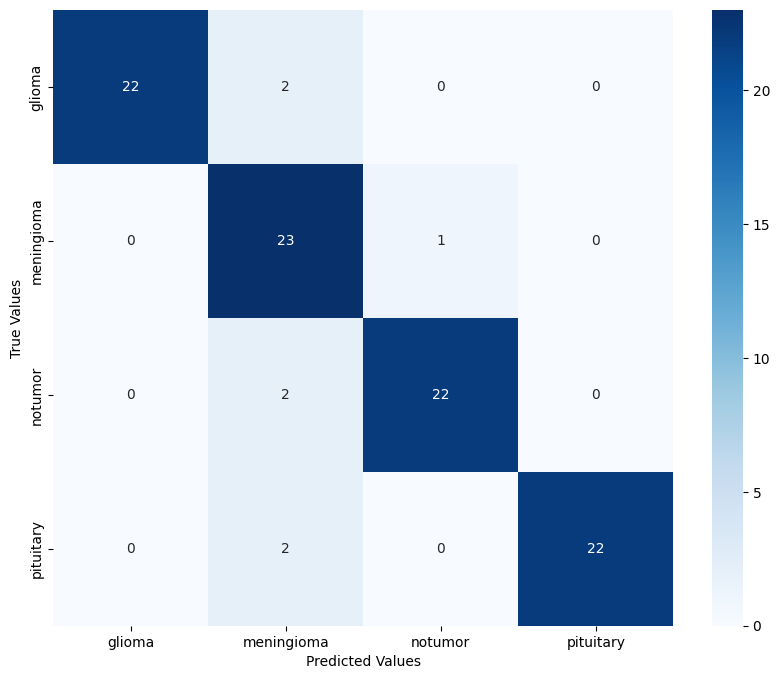
\includegraphics[width=\textwidth]{vit/vit_cm.png}
    \caption{Confusion Matrix}
    \label{fig:vit_cm}
  \end{subfigure}
  \hfill
  \begin{subfigure}[b]{0.2\textwidth}
    \centering
    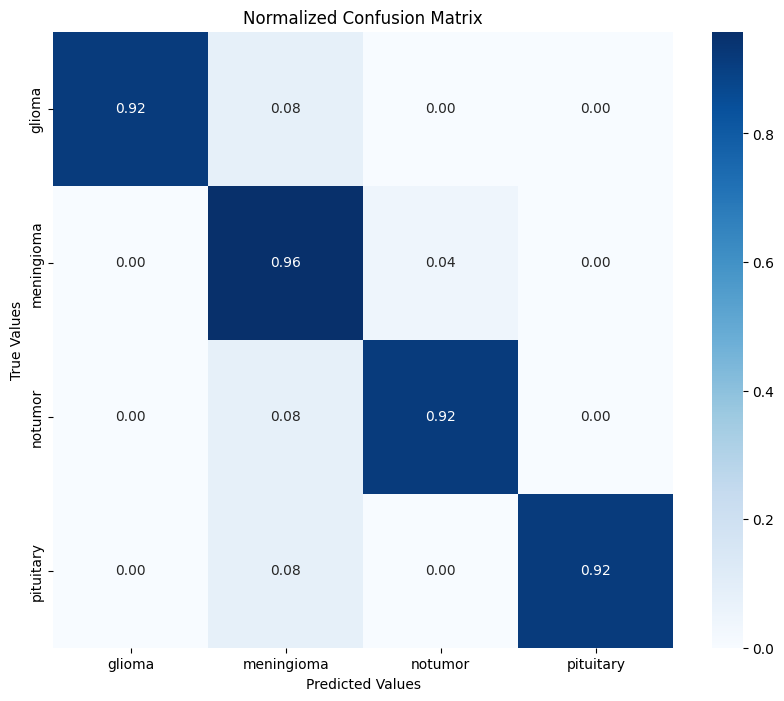
\includegraphics[width=\textwidth]{vit/vit_normcm.png}
    \caption{Normalized Confusion Matrix}
    \label{fig:vit_normcm}
  \end{subfigure}
  \hfill
  \begin{subfigure}[b]{0.25\textwidth}
    \centering
    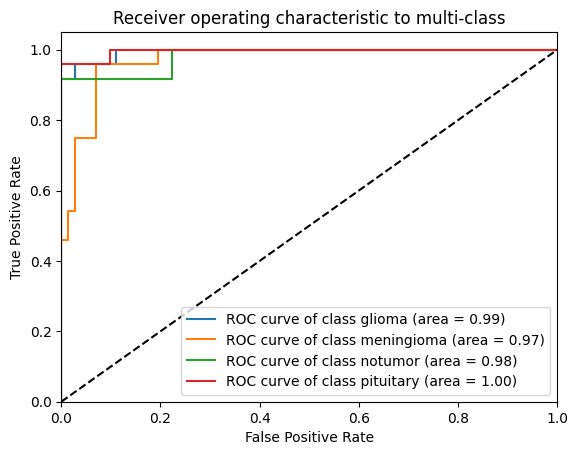
\includegraphics[width=\textwidth]{vit/vit_roc.png}
    \caption{ROC Curve}
    \label{fig:vit_roc}
  \end{subfigure}
  \hfill
  \begin{subfigure}[b]{0.25\textwidth}
    \centering
    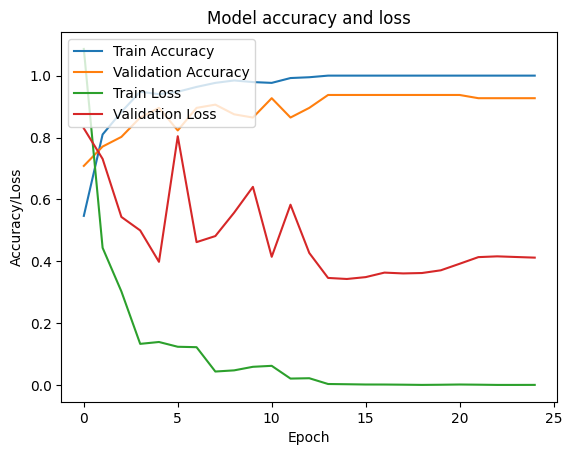
\includegraphics[width=\textwidth]{vit/vit_learningcurve.png}
    \caption{Learning Curve}
    \label{fig:vit_learning_curve}
  \end{subfigure}
  \caption{Confusion Matrix, Normalized Confusion Matrix, ROC Curve, and Learning Curve for Brain Tumor Segmentation}
  \label{fig:vit_evaluation}
\end{figure}

\begin{table}[ht]
\centering
\begin{tabular}{cc}
    \begin{minipage}{.6\linewidth}
        \centering
        \begin{subtable}[t]{\linewidth}
            \centering
            \begin{tabular}{|l|c|c|c|c|}
                \hline 
                \textbf{Class} & \textbf{Precision} & \textbf{Recall} & \textbf{F1-Score} & \textbf{Support} \\ 
                \hline 
                meningioma & 0.79 & 0.96 & 0.96 & 24 \\ 
                \hline
                pituitary  & 1.00 & 0.92 & 0.96 & 24 \\ 
                \hline
                glioma     & 1.00 & 0.92 & 0.96 & 24 \\ 
                \hline
                notumor    & 0.96 & 0.92 & 0.94 & 24 \\ 
                \hline
                micro avg  & 0.93 & 0.93 & 0.93 & 96 \\ 
                \hline
                macro avg  & 0.94 & 0.93 & 0.93 & 96 \\ 
                \hline
                weighted avg & 0.94 & 0.93 & 0.93 & 96 \\ 
                \hline
                samples avg & 0.93 & 0.93 & 0.93 & 96 \\ 
                \hline
            \end{tabular}
            \caption{Classification Report for Brain Tumor Segmentation} 
            \label{tab:vit_classification_report}
        \end{subtable}
    \end{minipage} &
    \begin{minipage}{.35\linewidth}
        \centering
        \begin{subtable}[t]{\linewidth}
            \centering
            \begin{tabular}{|c|c|}
                \hline 
                \textbf{Metric} & \textbf{Value} \\ 
                \hline
                DSC & 0.9293 \\ 
                \hline
                Sensitivity & 0.9271 \\ 
                \hline
                Specificity & 0.9757 \\ 
                \hline
                Accuracy & 0.9271 \\ 
                \hline
            \end{tabular}
            \caption{Additional Metrics for Brain Tumor Segmentation} 
            \label{tab:vit_additional_metrics}
        \end{subtable}
    \end{minipage}
\end{tabular}
\caption{Classification Report and Additional Metrics for Brain Tumor Segmentation using ViT}
\label{tab:combined_metrics}
\end{table}

The confusion matrices in Figures \ref{fig:vit_cm} and \ref{fig:vit_normcm} provide a detailed view of the model's performance across the four brain tumor classes: meningioma, pituitary, glioma, and no tumor. The classification report in Table \ref{tab:vit_classification_report} summarizes the precision, recall, and F1-score for each class. The model demonstrates high precision and recall across all classes, with notable F1-scores of 0.96 for meningioma, pituitary, and glioma classes. The overall micro, macro, and weighted averages for precision, recall, and F1-score all stand at 0.93, reflecting consistent and reliable performance.

The ROC curve in Figure \ref{fig:vit_roc} displays the true positive rate against the false positive rate for each class. The learning curve in Figure \ref{fig:vit_learning_curve} illustrates the model's accuracy and loss over multiple epochs, indicating effective learning without significant overfitting.

Table \ref{tab:vit_additional_metrics} highlights the Dice Similarity Coefficient (DSC), sensitivity, specificity, and accuracy of the model. The DSC of 0.9293 indicates a high overlap between the predicted and actual tumor regions. Sensitivity and accuracy, both at 0.9271, demonstrate the model's ability to correctly identify true positives, while the specificity of 0.9757 shows its effectiveness in correctly identifying true negatives.

\subsubsection{K-Folds Cross-Validation}

\begin{table}[H]
  \centering
  \caption{K-Folds Cross-Validation Testing Conditions}\label{tab:vit_kfolds_conditions}
  \begin{tabular}{cc}
      \begin{minipage}{.45\linewidth}
          \centering
          \begin{subtable}[t]{\linewidth}
              \centering
              \begin{tabular}{|l|c|}
                  \hline
                  \textbf{Parameter} & \textbf{Value} \\
                  \hline
                  Number of Folds ($k$) & 5 \\
                  \hline
                  Epochs & 20 \\
                  \hline
                  Batch Size & 16 \\
                  \hline
              \end{tabular}
              \caption{Training Parameters}
              \label{tab:vit_kfolds_parameters}
          \end{subtable}
      \end{minipage} &
      \begin{minipage}{.45\linewidth}
          \centering
          \begin{subtable}[t]{\linewidth}
              \centering
              \begin{tabular}{|l|c|}
                  \hline
                  \textbf{Metric} & \textbf{Value} \\
                  \hline
                  Average Validation Accuracy & 0.9542 \\
                  \hline
                  Average Validation Loss & 0.1880 \\
                  \hline
                  Validation Accuracy Std. Dev. & 0.0260 \\
                  \hline
                  Validation Loss Std. Dev. & 0.1124 \\
                  \hline
              \end{tabular}
              \caption{Evaluation Metrics}
              \label{tab:vit_kfolds_metrics}
          \end{subtable}
      \end{minipage}
  \end{tabular}
  \end{table}

To comprehensively evaluate the Vision Transformer (ViT) model's ability to generalize in the brain tumor segmentation task, K-Folds cross-validation was employed. The dataset was divided into five folds, with each fold taking a turn as the validation set while the remaining four folds were used for training. This process was repeated five times to ensure that each fold served as the validation set once, thus providing a thorough assessment of the model's performance. Each training session spanned 20 epochs, with model checkpoints removed for efficiency. The training parameters and evaluation metrics are summarized in Table \ref{tab:vit_kfolds_conditions}.

\begin{figure}[H]
  \centering
  \begin{subfigure}[b]{0.45\textwidth}
    \centering
    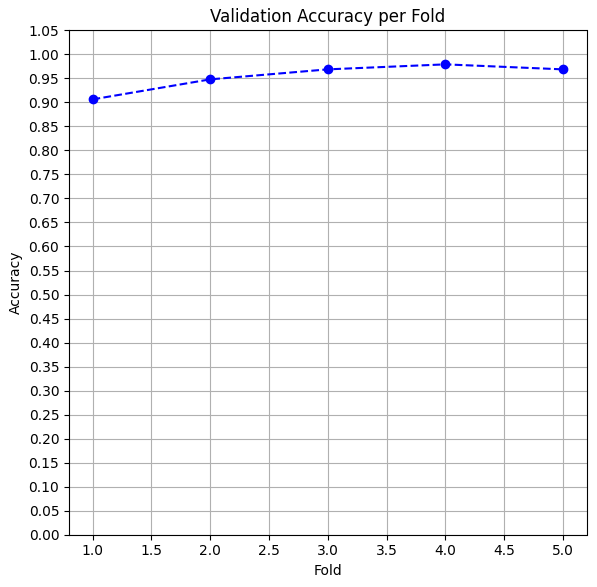
\includegraphics[width=\textwidth]{vit/vit_kfold_acc.png}
    \caption{Validation Accuracy per Fold}
    \label{fig:vit_accuracy}
  \end{subfigure}
  \hfill
  \begin{subfigure}[b]{0.45\textwidth}
    \centering
    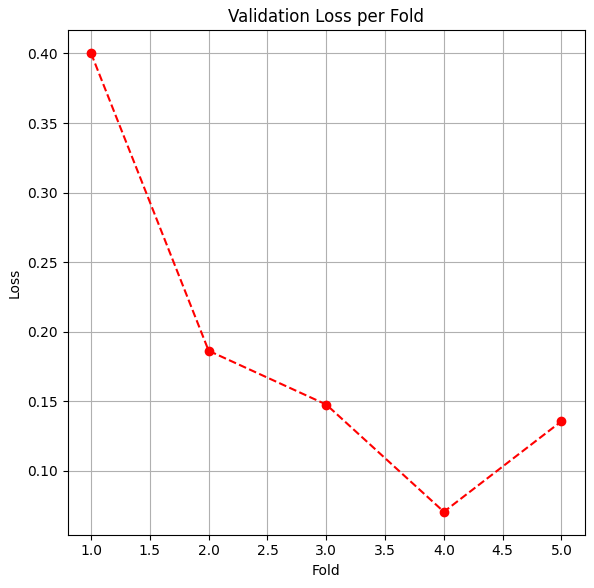
\includegraphics[width=\textwidth]{vit/vit_kfold_loss.png}
    \caption{Validation Loss per Fold}
    \label{fig:vit_loss}
  \end{subfigure}
  \caption{K-Folds Cross-Validation Results for ViT Model}
  \label{fig:vit_kfolds}
\end{figure}

The left plot in Figure \ref{fig:vit_accuracy} displays the validation accuracy for each fold. The results indicate consistently high performance across all folds, with accuracy values ranging from approximately 0.90 to 1.00. This demonstrates the model's strong capability in accurately segmenting brain tumors and suggests that it generalizes well to unseen data, maintaining robust performance across different data subsets.

The right plot in Figure \ref{fig:vit_loss} shows the validation loss for each fold, which exhibited more variability compared to the accuracy. The highest loss was observed in fold 1, while the lowest loss was seen in fold 4. This variability highlights areas where the model's performance can be further optimized to achieve more consistent results across different validation sets.

Interestingly, there were instances during the K-Folds validation where the validation loss was lower than the training's validation loss, and the validation accuracy was higher. This indicates the model's robustness and its ability to perform well on unseen data. However, this could also be due to variations in data distribution between the training and validation sets in each fold, which might result in slightly overestimated performance metrics. It is essential to consider these factors when interpreting the results.

Overall, the K-Folds cross-validation revealed that the model achieved a high average accuracy of 0.9542 with a standard deviation of 0.0260, indicating robust performance with minimal variability. The average validation loss was 0.1880 with a standard deviation of 0.1124, suggesting that while the model's predictions are generally reliable, there is room for improvement in reducing prediction errors. These findings demonstrate the model's strong generalization capabilities, although further refinement could enhance its consistency and reliability even more.


\subsubsection{Conclusion}

The Vision Transformer (ViT) model demonstrates significant potential in the domain of brain tumor segmentation from MRI scans. This study explored the adaptation of transformer architectures, originally designed for natural language processing, to visual data. The application of self-attention mechanisms allowed the ViT to dynamically prioritize different image segments, crucial for tasks like tumor detection in brain MRI scans.

Interestingly, the ViT model excelled in training directly with the original images without requiring extensive preprocessing. This ability to work effectively with raw images simplifies the preprocessing pipeline and saves computational resources, which is advantageous in practical applications. Despite the dataset's limitations, the ViT produced commendable results, showcasing its robustness and adaptability.

However, this study faced challenges due to the relatively small size of the training dataset. ViT models typically excel with large datasets, where they can fully leverage their capacity to learn complex patterns and subtle nuances. The small dataset limited the model's ability to generalize, which is evident from the variability observed in the validation losses across different folds. This limitation underscores the need for larger and more diverse datasets to fully realize the benefits of ViTs in medical imaging tasks.

K-Folds cross-validation was employed to assess the model's generalization performance rigorously. The dataset was divided into five folds, with each fold taking a turn as the validation set while the remaining four folds were used for training, repeated over 20 epochs per fold. The training parameters and evaluation metrics are summarized in Table \ref{tab:vit_kfolds_conditions}.

The cross-validation results, depicted in Figure \ref{vit_kfolds}, showed that the ViT model achieved an average validation accuracy of 0.9542 with a standard deviation of 0.0260. This high accuracy, coupled with minimal variability, suggests robust performance across different data subsets. However, the average validation loss of 0.1880 with a standard deviation of 0.1124 indicates room for improvement in reducing prediction errors. The variability in validation loss across folds points to the potential benefit of a larger training dataset to stabilize and enhance model performance further.

Despite the dataset constraints, the ViT model's performance is commendable, particularly in identifying complex patterns in medical images that are crucial for accurate diagnostics. Utilizing Optuna for hyperparameter optimization, the study found optimal learning and dropout rates, further enhancing the model's performance. These findings highlight the model's robustness and adaptability, making it a promising tool for medical diagnostics.

In summary, while the ViT model has shown excellent results in brain tumor segmentation, the small training set poses limitations on its generalization capability. Future work should focus on acquiring larger datasets and exploring advanced data augmentation techniques to improve model robustness and reliability. Additionally, continued refinement of preprocessing steps and fine-tuning parameters will further enhance the ViT model's applicability in clinical settings.

